\documentclass[12pt,a4paper]{article}
\usepackage[utf8]{inputenc}
\usepackage[margin=2.5cm, top=2.5cm, includefoot]{geometry}
\usepackage[spanish]{babel}
\usepackage{amsmath}
\usepackage{amsfonts}
\usepackage{amssymb}
\usepackage{graphicx}
\usepackage[table,xcdraw]{xcolor}
\usepackage[most]{tcolorbox}
\usepackage{fancyhdr}
\usepackage{multicol}

\author{Ronald Ari}
\title{Propiedades de los Límites }
\date{\today}

%Colores
\definecolor{violeta}{HTML}{4b31de}

%arriba de página
\setlength{\headheight}{40pt}
\pagestyle{fancy}
\fancyhf{}
\lhead{{\large \textbf {Ronald Ari}}}
\rhead{
\includegraphics[width=2.5cm]{imagenes/logo_unaj.png}}
\chead{{\large \textbf{Cálculo Diferencial}}}

%Inicio del documento ------------------------------------------

\begin{document}

    \begin{titlepage}
    \centering
    
\includegraphics[width=\textwidth,height=5cm,keepaspectratio]{imagenes/logo_unaj.png}\par\vspace{1cm}
    {\Huge\textbf{Cálculo Diferencial}\par\vspace{0.4cm}}
    {\Huge\textbf{Formulario}\par\vspace{1cm}}
    {\Huge\bfseries\textcolor{violeta}{\textbf{Límites Matemáticos}}} \par\vspace{2cm}
    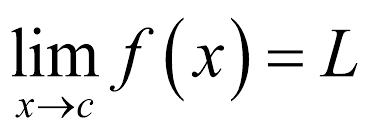
\includegraphics[width=\textwidth,height=10cm,keepaspectratio]{imagenes/limites.png}\par\vspace{1cm}
    \vfill{}
    \begin{tcolorbox}[colback=white!5!white,colframe=blue!75!black]
        \centering
        {\Huge\textbf{De:}} {\LARGE\textbf{Ronald Francisco Ari Paredes}}
    \end{tcolorbox}
    \vfill
    {\Large\today}
    \end{titlepage}
    %------------------------------------------------------------
    \clearpage
    \section{\textcolor{violeta}{Límites y límites laterales}}
    \begin{tcolorbox}[colback=white!5!white,colframe=violeta!75!black]
        \begin{enumerate}
        \centering
        \item $\displaystyle\lim_{x \to {c^+}}{f(x)}=\displaystyle\lim_{x \to {c^-}}{f(x)}=L\Leftrightarrow \displaystyle\lim_{x \to c}{f(x)}=L $
        \item $\displaystyle\lim_{x \to {c^+}}{f(x)}\neq \displaystyle\lim_{x \to {c^-}}{f(x)} \Rightarrow  \nexists\lim_{x \to c}{f(x)}  $
        \end{enumerate}
    \end{tcolorbox}

    \section{\textcolor{violeta}{Límites de funciones simples}}
    \begin{tcolorbox}[colback=white!5!white,colframe=violeta!75!black]
        \begin{multicols}{2}
            \begin{enumerate}
                \item $\displaystyle\lim_{x \to c}{a}=a $
                \item $\displaystyle\lim_{}{} $
                \item $\displaystyle\lim_{x \to c}{ax+b}=ac+b $
                \item $\displaystyle\lim_{x \to c}{x^r}=c^r $ 
                \item $\displaystyle\lim_{x \to {0^+}}{\frac{1}{x^r}}=+\infty $
                \item $\displaystyle\lim_{x \to {0^-}}{\frac{1}{x^r}}=\left\lbrace \begin{array}{c} -\infty\:;\:Si\:r\:es\:impar\\+\infty\:;\:Si\:r\:es\:par \end {array} \right. $ 
            \end{enumerate}
        \end{multicols}
    \end{tcolorbox}

    \section{\textcolor{violeta}{Hechos sobre $\pm\infty$ en Límites}}
    \begin{tcolorbox}[colback=white!5!white,colframe=violeta!75!black]
        \begin{multicols}{2}
            \begin{enumerate}
                \item Si $a\neq0 $ y $a<\infty$:\\
                $\circ\:0+\infty=\infty$\\
                $\circ\:a+\infty=\infty$\\
                $\circ\:\frac{a}{\infty}=0 $\\
                $\circ\:\frac{a}{0}=\left\lbrace\begin{array}{c}\infty,\:a>0\\-\infty,\:a<0\end {array} \right. $\\
                $\circ\:a\times\infty=\left\lbrace\begin{array}{c}\infty,\:a>0\\-\infty,\:a<0\end {array} \right. $
            \end{enumerate}            
        \end{multicols}
    \end{tcolorbox}

    \section{\textcolor{violeta}{Hechos sobre funciones}}
    \begin{tcolorbox}[colback=white!5!white,colframe=violeta!75!black]
        \begin{enumerate}
            \begin{multicols}{2}
                \item $\displaystyle\lim_{x\to0}{sen (x)}=sen (0)=0 $
                \item $\displaystyle\lim_{x\to0}{\cos(x)}=\cos(0)=1 $
                \item $\displaystyle\lim_{x\to{a}}{sen (x)}=sen (a) $
                \item $\displaystyle\lim_{x\to{a}}{\cos(x)}=\cos(a) $
                \item $\displaystyle\lim_{x\to0}{e^x}=e^0=1 $
                \item $\displaystyle\lim_{x\to{a}}{\log_a (a)}=1 $
            \end{multicols}
            \centering
            \item Si $a>1 $\\ \vspace{0.5cm}
            $\circ\displaystyle\lim_{z\to{0^+}}{\log_ax}=\displaystyle\lim_{z\to{0^+}}{\ln{x}}=\displaystyle\lim_{x\to{0^+}}{\log_{10}{x}}=-\infty$\\ \vspace{0.4cm}
            $\circ\displaystyle\lim_{z\to{\infty}}{\log_ax}=\displaystyle\lim_{z\to{\infty}}{\ln{x}}=\displaystyle\lim_{x\to{\infty}}{\log_{10}{x}}=\infty$
            \item Si $a<1 $\\ \vspace{0.1cm}
            \begin{multicols}{2}
                $\circ\displaystyle\lim_{z\to{0^+}}{\log_a{x}}=\infty$\\
                $\circ\displaystyle\lim_{z\to{\infty}}{\log_a{x}}=-\infty$
            \end{multicols}
        \end{enumerate}        
    \end{tcolorbox}

    \pagebreak

    \section{\textcolor{violeta}{Formas Indeterminadas}}
    \begin{tcolorbox}[colback=white!5!white,colframe=violeta!75!black]
        \centering
        $\frac{0}{0},\:\frac{\infty}{\infty},\:0\times\infty,\:1^{\infty},\:\infty-\infty,\:0^0\:y\:\infty^0 $
    \end{tcolorbox}

    \section{\textcolor{violeta}{Formas no Indeterminadas}}
    \begin{tcolorbox}[colback=white!5!white,colframe=violeta!75!black]
        \begin{enumerate}
            \begin{multicols}{2}
                \item Si $\displaystyle\lim_{z\to{c}}{\frac{f (x)}{g (x)}} $ tiene la forma $\left[\frac{1}{0}\right]$: \\ 
                $\displaystyle\lim_{z\to{c}}{\frac{f (x)}{g (x)}}=\left\lbrace\begin{array}{c}-\infty\\+\infty\\No\:existe\end{array} \right. $
                \item Si $\displaystyle\lim_{x\to{c}}{f (x)^{g (x)}} $ tiene la forma $\left[0^{\infty}\right]$: \\ 
                $\displaystyle\lim_{z\to{c}}{f (x)^{g (x)}}=0$
            \end{multicols}
        \end{enumerate}
    \end{tcolorbox}

    \section{\textcolor{violeta}{Límites cerca de Infinito}}
    \begin{tcolorbox}[colback=white!5!white,colframe=violeta!75!black]
        \begin{enumerate}
            \begin{multicols}{2}
                \item $\displaystyle\lim_{x\to{\infty}}{\frac{a}{x}}=0, $ para todo real a
                \item $\displaystyle\lim_{x\to{\infty}}{\sqrt[x]{x}}=1 $                
                \item $\displaystyle\lim_{x\to{\infty}}{\sqrt[a]{x}}=1 $
                \item $\displaystyle\lim_{x\to{\infty}}{\infty} $ para todo $a>0 $
                \item $\displaystyle\lim_{x\to{\infty}}{\frac{x}{a}}=\left\lbrace\begin{array}{c}\infty,\hspace{1.3cm}a>0\\no\:existe,\:a=0\\-\infty,\hspace{1cm}a<0\end{array} \right. $
                \item $\displaystyle\lim_{z\to{\infty}}{X^a}=\left\lbrace\begin{array}{c}\infty,\hspace{1.1cm}a>0\\1,\hspace{1.3cm}a=0\\0,\hspace{1.4cm}a<0\end{array} \right. $
                \item $\displaystyle\lim_{x\to{\infty}}{a^x}=\left\lbrace\begin{array}{c}\infty,\hspace{1.3cm}a>0\\1,\hspace{1.5cm}a=0\\0,\hspace{0.8cm}0<a<1\end{array} \right. $
                \item $\displaystyle\lim_{x\to{\infty}}{a^{-x}}=\left\lbrace\begin{array}{c}0,\hspace{1.5cm}a>0\\1,\hspace{1.5cm}a=0\\\infty,\hspace{0.6cm}0<a<1\end{array} \right. $
            \end{multicols}            
        \end{enumerate}
    \end{tcolorbox}

    \section{\textcolor{violeta}{Límites de Polinomios}}
    \begin{tcolorbox}[colback=white!5!white,colframe=violeta!75!black]
        \centering
        $\displaystyle\lim_{z\to{\infty}}\left[a_nX^n+...+a_1\right]=\displaystyle\lim_{z\to{\infty}}{a_nX^n}\hspace{1cm} $ $\leftarrow$ Máxima potencia. \\ \vspace{0.5cm}
        $\displaystyle\lim_{z\to{\infty}}{\frac{mx^a}{nx^b}}=\left\lbrace\begin{array}{c}0,\hspace{1.2cm}Si\:a<b\\\frac{m}{n},\hspace{1.1cm}Si\:a=b\\\infty,\hspace{1cm}Si\:a>b\end{array} \right.  $
    \end{tcolorbox}

    \section{\textcolor{violeta}{Límites de funciones generales}}
    \begin{tcolorbox}[colback=white!5!white,colframe=violeta!75!black]
        \begin{enumerate}
            \centering
            \item Si: $\hspace{0.5cm}\displaystyle\lim_{x\to{c}}{f (x)}=F $ y $\displaystyle\lim_{z\to{c}}{g (x)}=G \hspace{0.5cm}$ Entonces:
            \begin{multicols}{2}
                \begin{itemize}
                    \item $\displaystyle\lim_{x\to{c}}{\left[f (x)\pm{g (x)}\right]}=F\pm{G} $
                    \item $\displaystyle\lim_{x\to{c}}{\left[a\times{g (x)}\right]}=a\times{G} $
                \end{itemize}
            \end{multicols}            
        \end{enumerate}
    \end{tcolorbox}
    \begin{tcolorbox}[colback=white!5!white,colframe=violeta!75!black]
        \begin{multicols}{2}
            \centering
            \begin{itemize}
                \item $\displaystyle\lim_{x\to{c}}{\left[f (x)\times{g (x)}\right]}=F\times{G} $
                \item $\displaystyle\lim_{x\to{c}}{\frac{f (x)}{g (x)}}=\frac{F}{G} $
                \item $\displaystyle\lim_{x\to{c}}{f (x)^n}=F^n $
                \item $\displaystyle\lim_{x\to{c}}{\sqrt[n]{f (x)}}=\sqrt[n]{F} $
            \end{itemize}
         \end{multicols}            
    \end{tcolorbox}
    
    \section{\textcolor{violeta}{Composición de funciones}}
    \begin{tcolorbox}[colback=white!5!white,colframe=violeta!75!black]
        \begin{enumerate}
            \item Si $f (x)$ es continua $\displaystyle\lim_{z\to{c}}{g (x)}=G $ Entonces:
        \end{enumerate}
        \centering
        $\displaystyle\lim_{x\to{c}}{f (g (x))}=f (\displaystyle\lim_{z\to{c}}{g (x)})=f (G) $
    \end{tcolorbox}

    \section{\textcolor{violeta}{Límites y Derivadas}}
    \begin{tcolorbox}[colback=white!5!white,colframe=violeta!75!black]
        \begin{enumerate}
            \begin{multicols}{2}
                \item $\displaystyle\lim_{h\to{0}}{\frac{f (x+h)-f (x)}{h}}=f' (x) $
                \item $\displaystyle\lim_{h\to{x}}{\sqrt[n]{\frac{f (x+h)}{f (x)}}}=\exp\left(\frac{f' (x)}{f (x)}\right) $                
                \item $\displaystyle\lim_{h\to{0}}{\sqrt[n]{\frac{f (x+h\times{x})}{f (x)}}}=\exp\left(\frac{xf' (x)}{f (x)}\right) $
            \end{multicols}            
        \end{enumerate}
    \end{tcolorbox}

    \section{\textcolor{violeta}{Límites en Funciones Trigonométricas}}
    \begin{tcolorbox}[colback=white!5!white,colframe=violeta!75!black]
        \begin{enumerate}
            \begin{multicols}{2}
                \item $\displaystyle\lim_{x\to{0}}{\frac{\sin(x)}{x}}=1 $
                \item $\displaystyle\lim_{x\to{0}}{\frac{\sin(ax)}{ax}}=1 $, para $a\neq0 $
                \item $\displaystyle\lim_{x\to{0}}{\frac{1-\cos(x)}{x}}=1 $
                \item $\displaystyle\lim_{x\to{0}}{\frac{1-\cos(x)}{x^2}}=\frac{1}{2} $
                \item $\displaystyle\lim_{x\to{n^{\pm}}}{\tan\left(\pi{x}+\frac{\pi}{2}\right)}=\pm\infty$, para $n\epsilon\mathbb{Z} $
                \item $\displaystyle\lim_{x\to{0}}{\frac{\sin(ax)}{x}}=a $ 
                \item $\displaystyle\lim_{x\to{0}}{\frac{\sin(ax)}{bx}}=\frac{a}{b} $, para $b\neq{0}$
            \end{multicols}
        \end{enumerate}
    \end{tcolorbox}

    \section{\textcolor{violeta}{Límites Especiales Notables}}
    \begin{tcolorbox}[colback=white!5!white,colframe=violeta!75!black]
    \begin{enumerate}
        \begin{multicols}{3}
           \item $\displaystyle\lim_{x\to{0^+}}{x^x}=1 $
           \item $\displaystyle\lim_{x\to{0}}{\left(1+x\right)^{\frac{1}{x}}}=e $
           \item $\displaystyle\lim_{x\to{+\infty}}{\left(1+\frac{1}{x}\right)^x} $
           \item $\displaystyle\lim_{x\to{\infty}}{\frac{n}{\sqrt[n]{n!}}}=e $
           \item $\displaystyle\lim_{x\to{+\infty}}{\left(1-\frac{1}{x}\right)^x}=\frac{1}{e} $
           \item $\displaystyle\lim_{x\to{+\infty}}{\left(1+\frac{k}{x}\right)^{mx}}=e^{mx} $
        \end{multicols}
    \end{enumerate}
    \end{tcolorbox}
    \begin{tcolorbox}[colback=white!5!white,colframe=violeta!75!black]
        \begin{enumerate}
            \begin{multicols}{3}
                \setcounter{enumi}{6}
                \item $\displaystyle\lim_{x\to{+\infty}}{\left(\frac{x}{x+k}\right)^x}=\frac{1}{e^k} $
                \item $\displaystyle\lim_{x\to{0}}{\frac{a^x-1}{x}}=\ln(a) $
                \item $\displaystyle\lim_{x\to{0}}{\frac{c^{ax}-1}{bx}}=\frac{a}{b}\ln(c) $
                \item $\displaystyle\lim_{x\to{0}}{\frac{\sin(x)}{x}}=1 $
                \item $\displaystyle\lim_{x\to{0}}{\frac{\sin(x)}{x}}=1 $
                \item $\displaystyle\lim_{x\to{0}}{\frac{\cos(x)-1}{x}}=0 $
                \item $\displaystyle\lim_{x\to{0}}{\frac{(1+x)^n-1}{x}}=n $
                \item $\displaystyle\lim_{x\to{0}}{\frac{x^n-a^n}{x-a}}=0 $
                \item $\displaystyle\lim_{x\to{0}}{\frac{e^x-1}{x}}=1 $
                \item $\displaystyle\lim_{x\to{0}}{\frac{e^{ax}-1}{bx}}=\frac{a}{b} $
            \end{multicols} 
            \centering
                \item $\displaystyle\lim_{x\to{0}}{\left(1+a (e^{-x}-1)\right)^{\frac{-1}{x}}}=e^a $   
        \end{enumerate}
    \end{tcolorbox}

    \section{\textcolor{violeta}{Límetes en Logaritmos y exponentes}}
    \begin{tcolorbox}[colback=white!5!white,colframe=violeta!75!black]
        \begin{enumerate}
            \begin{multicols}{2}
                \item $\displaystyle\lim_{x\to{\infty}}{xe^{-z}}=0 $
                \item $\displaystyle\lim_{x\to{1}}{\frac{\ln(x)}{x-1}}=1 $
                \item $\displaystyle\lim_{x\to{0}}{\frac{\ln(x+1)}{x}}=1 $ 
                \item $\displaystyle\lim_{x\to{0}}{\frac{\ln(1+ax)}{bx}}=\frac{a}{b} $
                \item $\displaystyle\lim_{x\to{0}}{\frac{\log_c (1+ax)}{bx}}=\frac{a}{b\ln{c}} $
                \item $\displaystyle\lim_{x\to{0}}{\frac{-\ln(1+a\times(e^{-x}-1))}{x}}=a $
            \end{multicols}
        \end{enumerate}
    \end{tcolorbox}


    
\end{document}